\documentclass{article}

\usepackage{graphicx}
\usepackage[hidelinks]{hyperref}
\usepackage[a4paper, total={6in, 8in}]{geometry}
\usepackage[slovak]{babel}
\usepackage{caption}
\usepackage{subcaption}
\usepackage{listings}

\graphicspath{./include/}

\renewcommand{\figurename}{Obr.}
\renewcommand{\contentsname}{Obsah}
\captionsetup[table]{name=Tab.}

\begin{document}

\begin{titlepage}
	\null\vfill

	\begin{center}
		{\Huge Magnetická levitácia }
		\vskip 2cm

		{\Large Cvičenie č. 8}
		\vskip 0.5cm

		{\large Spojité procesy}
	\end{center}

	\vfill
	\vfill

	\begin{flushright}
		Filip Lobpreis \\
		Matúš Machata \\
		\small\today\\
	\end{flushright}
	\hfill
\end{titlepage}

\thispagestyle{empty}
\clearpage

\tableofcontents
\thispagestyle{empty}
\clearpage

\section{Zadanie}
\label{sec:zadanie}

\begin{figure}[!htbp]
	\begin{center}
		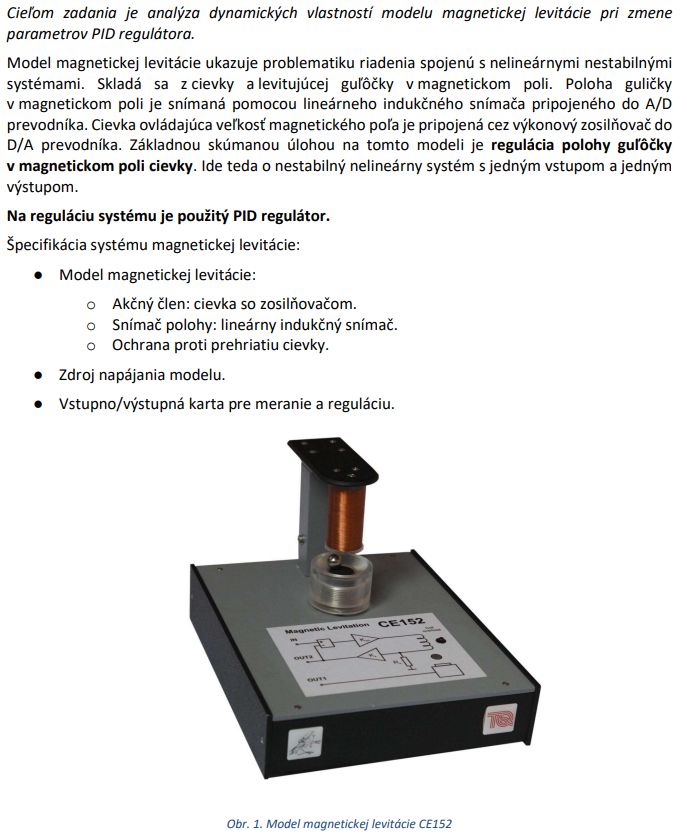
\includegraphics[width=0.95\textwidth]{include/zadanie.png}
	\end{center}
	\caption{Zadanie č. 8 z~predmetu Spojité procesy.}
	\label{fig:zadanie}
\end{figure}

\pagenumbering{arabic}
\clearpage

\section{Merania}
\label{sec:merania}

Ôsme zadanie z~predmetu spojité procesy sa zaoberá skúmaním vplyvu zmien koeficientov PID regulátora
na~ovládanie magnetickej levitácia. V~tomto zadaní budeme postupne meniť PID regulátor a~jeho \textbf{Proporcionálnu},
\textbf{Integračnú} a~\textbf{Derivačnú} zložku. Na~obrázku Obr.~\ref{fig:schema} vidíme model magnetickej levitácia,
ktorý sme použili pri~meraniach. Jednotlive parametre regulatora budeme menit v~rozsahu $\pm20\%$.

\begin{figure}[!htbp]
	\begin{center}
		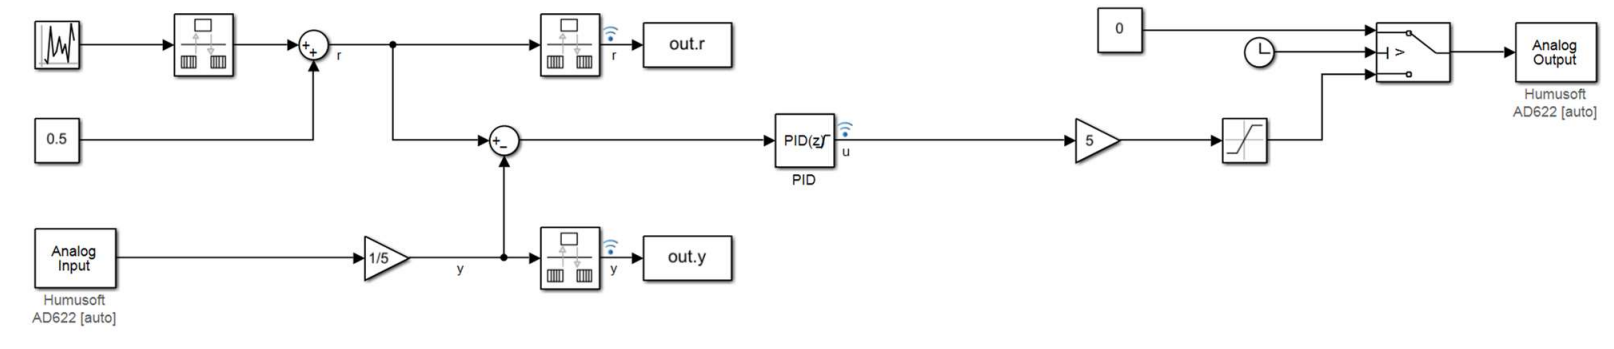
\includegraphics[width=0.95\textwidth]{include/schema.png}
	\end{center}
	\caption{Schéma pre~model magnetickej levitácie.}
	\label{fig:schema}
\end{figure}

\begin{table}[!htbp]
	\caption{Koeficienty PID regulatora}
	\label{tab:t0}
	\begin{center}
		\begin{tabular}[c]{|l|l|}
			\hline

			P & 1 \\
			I & 4 \\
			D & 0.016 \\
			\hline
		\end{tabular}
	\end{center}
\end{table}

\begin{figure}[!htbp]
	\begin{center}
		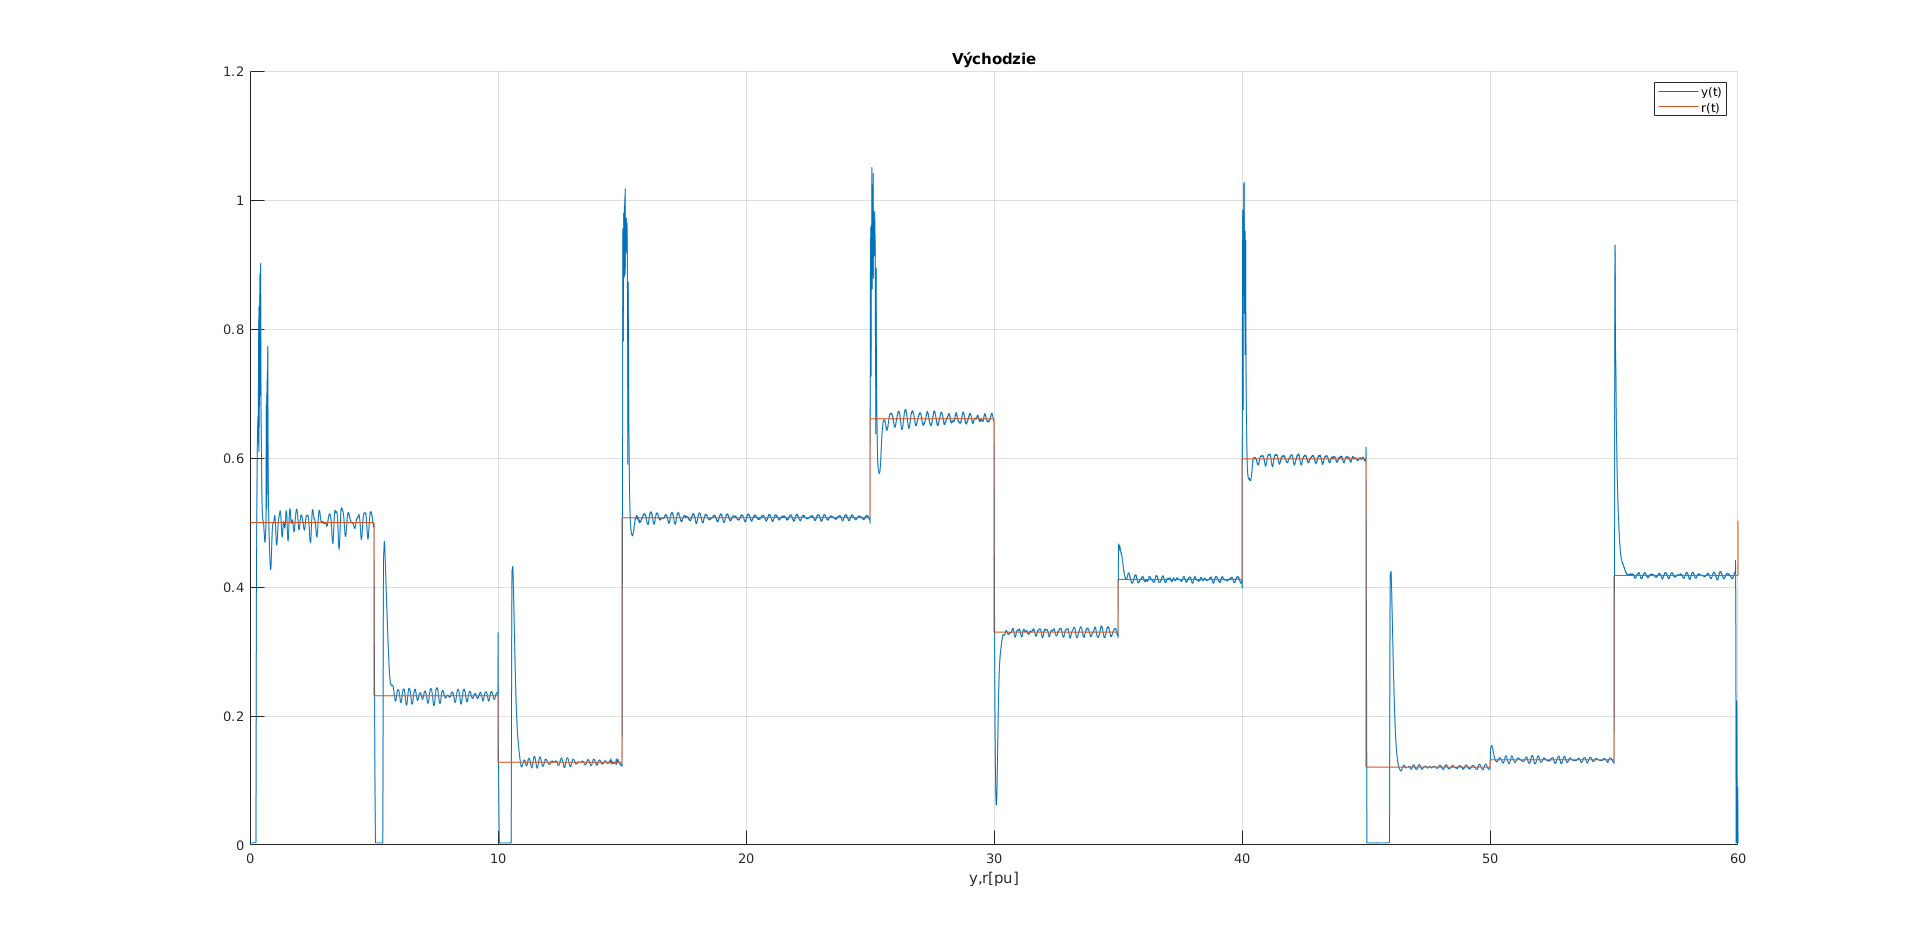
\includegraphics[width=0.95\textwidth]{include/m1.png}
	\end{center}
	\caption{Zakladne hodnoty PID regulatora.}
	\label{fig:m1}
\end{figure}

Obrázok Obr.~\ref{fig:m1} zobrazuje kmitavý tlmený proces s~preregulovaním. Môžeme vidieť, že~čím vysie mal
regulátor udržať kovovú guľôčku, tým viac bol systém rozkmitaný. Pri~prvých pätnástich sekundách merania
magnetické pole nedokázalo dostatočne stabilizovať guľôčku a~nastaval veľký rozkmit v~ustálenej hodnote.

\clearpage

\subsection{Meranie 1}
\label{sec:meranie1}

\begin{table}[!htbp]
	\caption{Koeficienty PID regulátora}
	\label{tab:t1}
	\begin{center}
		\begin{tabular}[c]{|l|l|}
			\hline
			P & 1.2 \\
			I & 4 \\
			D & 0.016 \\
			\hline
		\end{tabular}
	\end{center}
\end{table}

\begin{figure}[!htbp]
	\begin{center}
		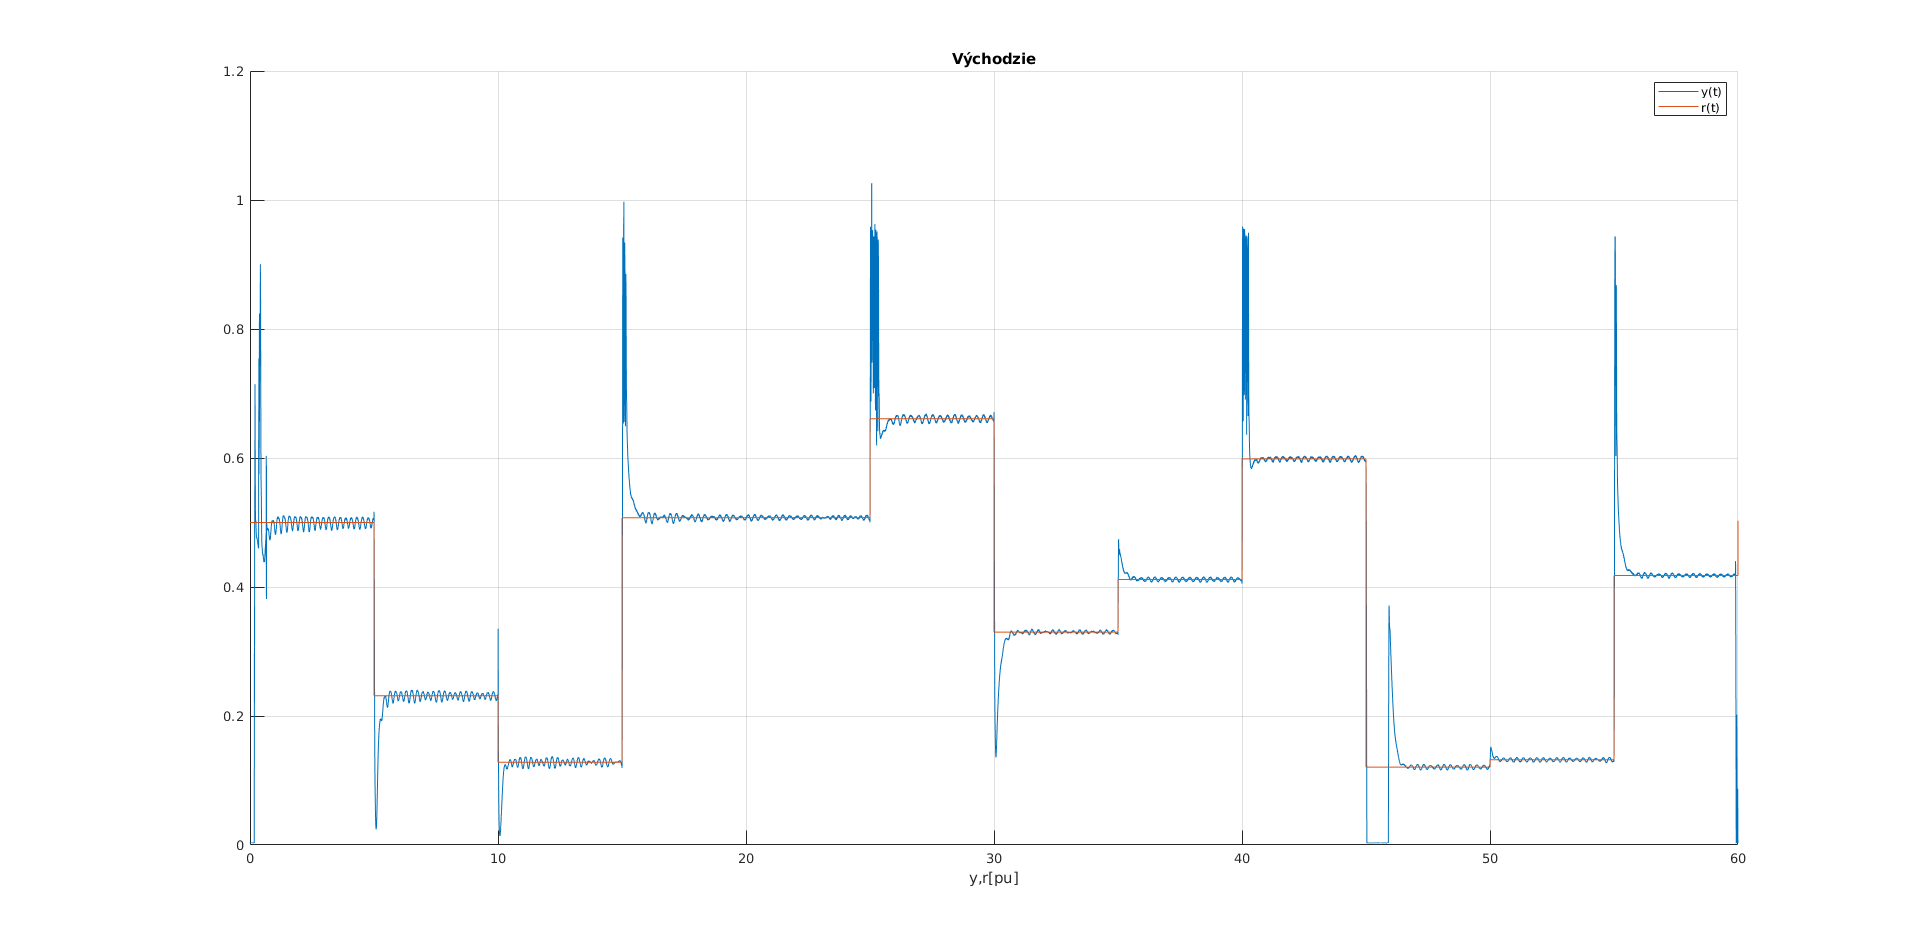
\includegraphics[width=0.8\textwidth]{./include/m2.png}
	\end{center}
	\caption{Graf prveho merania.}
	\label{fig:meranie1}
\end{figure}

V~prvom meraní sme zvesili \textbf{proporcionálnu} zložku regulátora o~20\%. Výsledok je viditeľný
na~obrázku Obr.~\ref{fig:meranie1}. Taktiež ako v~predchádzajúcom meraní bolo prvých pätnásť sekúnd
merania rozkmitaných. V~ďalších skokoch vidíme väčší účinok derivačnej zložky. Toto spôsobilo zvýšenie
už~spomenutej proporcionálnej zložky.

\clearpage

\subsection{Meranie 2}
\label{sec:meranie2}

\begin{table}[!htbp]
	\caption{Koeficienty PID regulátora}
	\label{tab:t2}
	\begin{center}
		\begin{tabular}[c]{|l|l|}
			\hline
			P & 0.8 \\
			I & 4 \\
			D & 0.016 \\
			\hline
		\end{tabular}
	\end{center}
\end{table}

\begin{figure}[!htbp]
	\begin{center}
		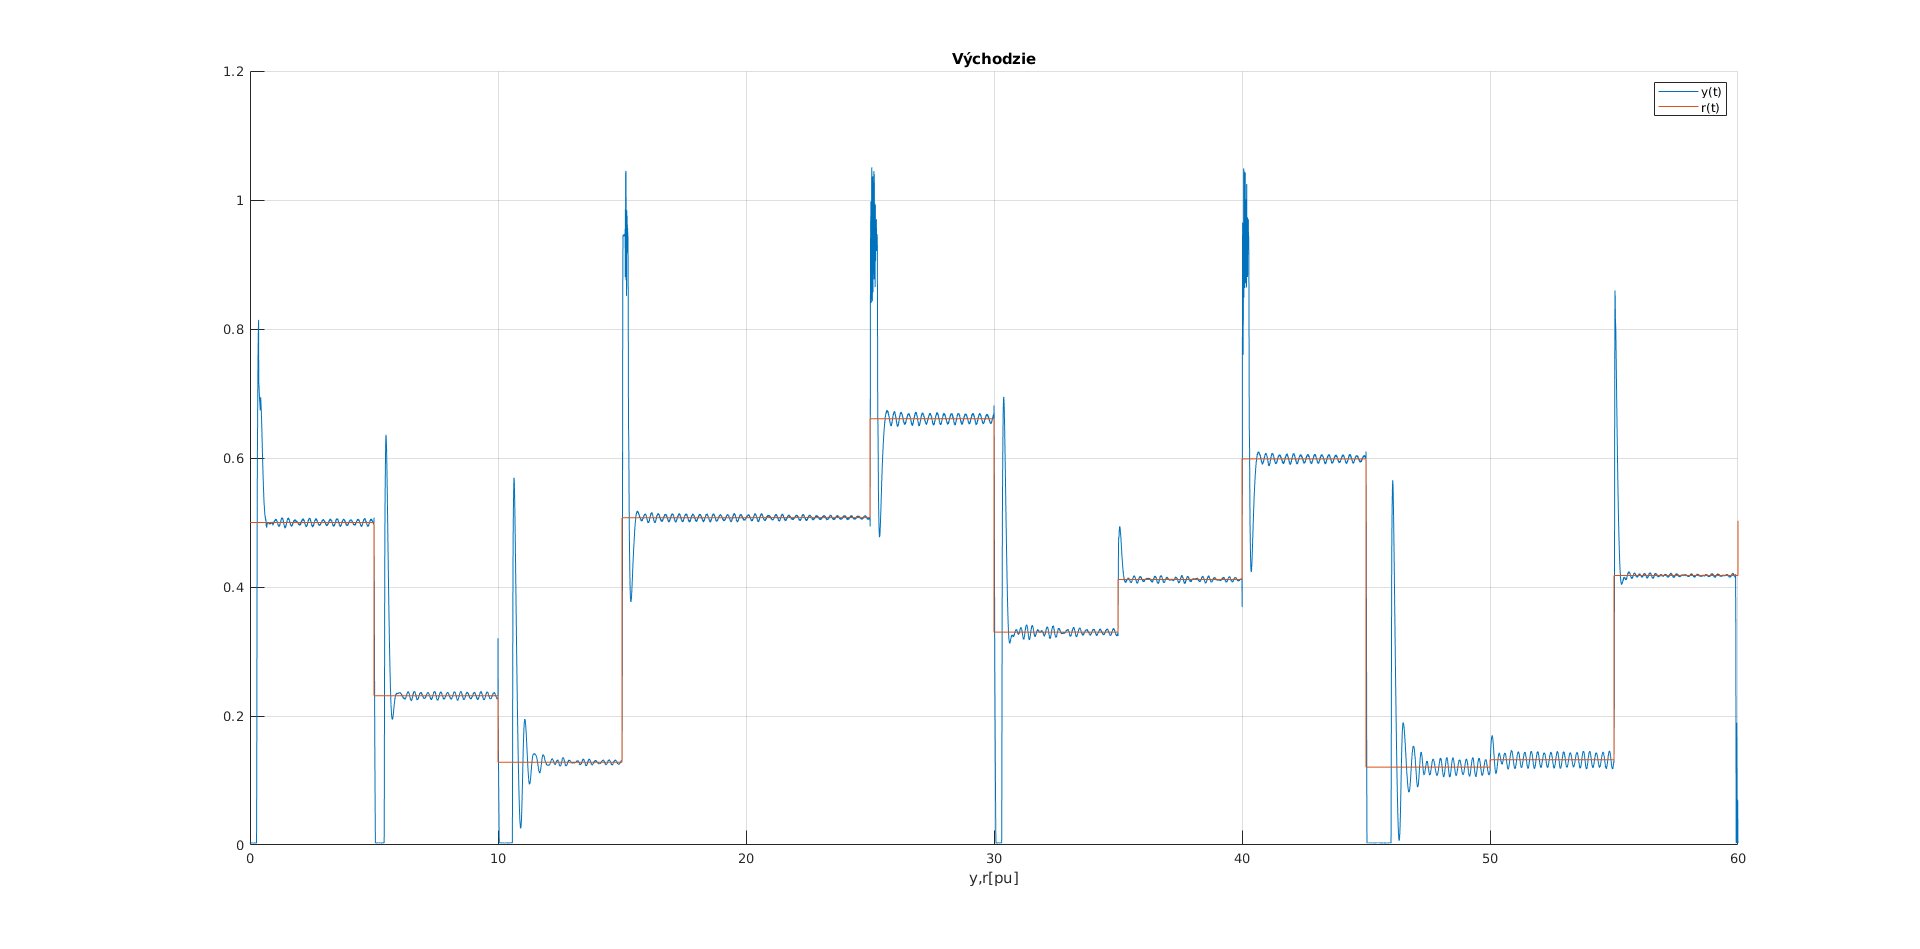
\includegraphics[width=0.8\textwidth]{./include/m3.png}
	\end{center}
	\caption{Graf druhého merania.}
	\label{fig:meranie2}
\end{figure}

V~druhom meraní sme zmenšili \textbf{proporcionálnu} zložku regulátora o~20\%. Výsledok je viditeľný
na~obrázku Obr.~\ref{fig:meranie2}. Taktiež ako v~predchádzajúcom meraní bolo prvých pätnásť sekúnd
merania rozkmitaných s~tým rozdielom, že~zmenšenie proporcionálnej zložky malo za~dôsledok menšiu
stabilitu systému pri~zmenšenie žiadanej hodnoty.

\clearpage

\subsection{Meranie 3}
\label{sec:meranie3}

\begin{table}[!htbp]
	\caption{Koeficienty PID regulátora}
	\label{tab:t3}
	\begin{center}
		\begin{tabular}[c]{|l|l|}
			\hline
			P & 1 \\
			I & 4.8 \\
			D & 0.016 \\
			\hline
		\end{tabular}
	\end{center}
\end{table}

\begin{figure}[!htbp]
	\begin{center}
		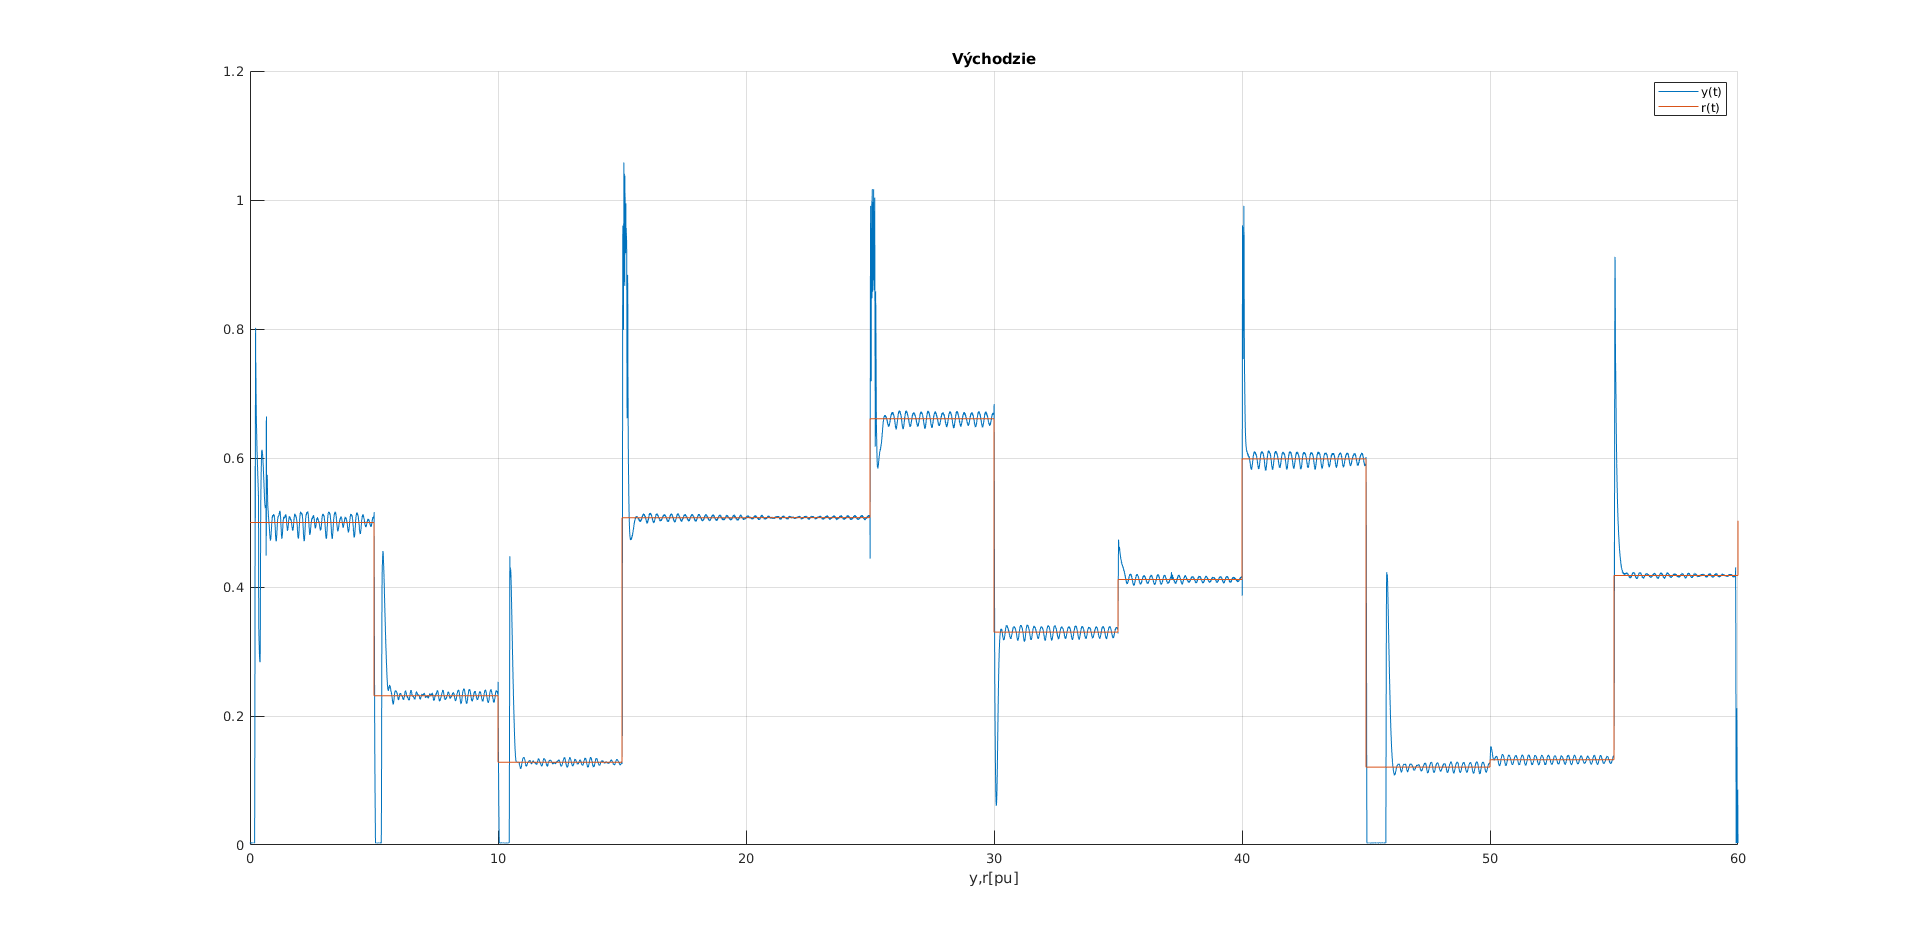
\includegraphics[width=0.8\textwidth]{./include/m4.png}
	\end{center}
	\caption{Graf tretieho merania.}
	\label{fig:meranie3}
\end{figure}

V~tretom meraní sme zväčšili \textbf{integračnú} zložku regulátora o~20\%. Výsledok je viditeľný
na~obrázku Obr.~\ref{fig:meranie3}. Zvýšenie integračnej zložky malo za~dôsledok rýchlejší stabilizáciu
systému. Ak~si všimneme úsek od~40 sekúnd po~45 sekúnd, vidíme, že~systém je na~hranici stability.

\clearpage

\subsection{Meranie 4}
\label{sec:meranie4}

\begin{table}[!htbp]
	\caption{Koeficienty PID regulátora}
	\label{tab:t4}
	\begin{center}
		\begin{tabular}[c]{|l|l|}
			\hline
			P & 1 \\
			I & 3.2 \\
			D & 0.016 \\
			\hline
		\end{tabular}
	\end{center}
\end{table}

\begin{figure}[!htbp]
	\begin{center}
		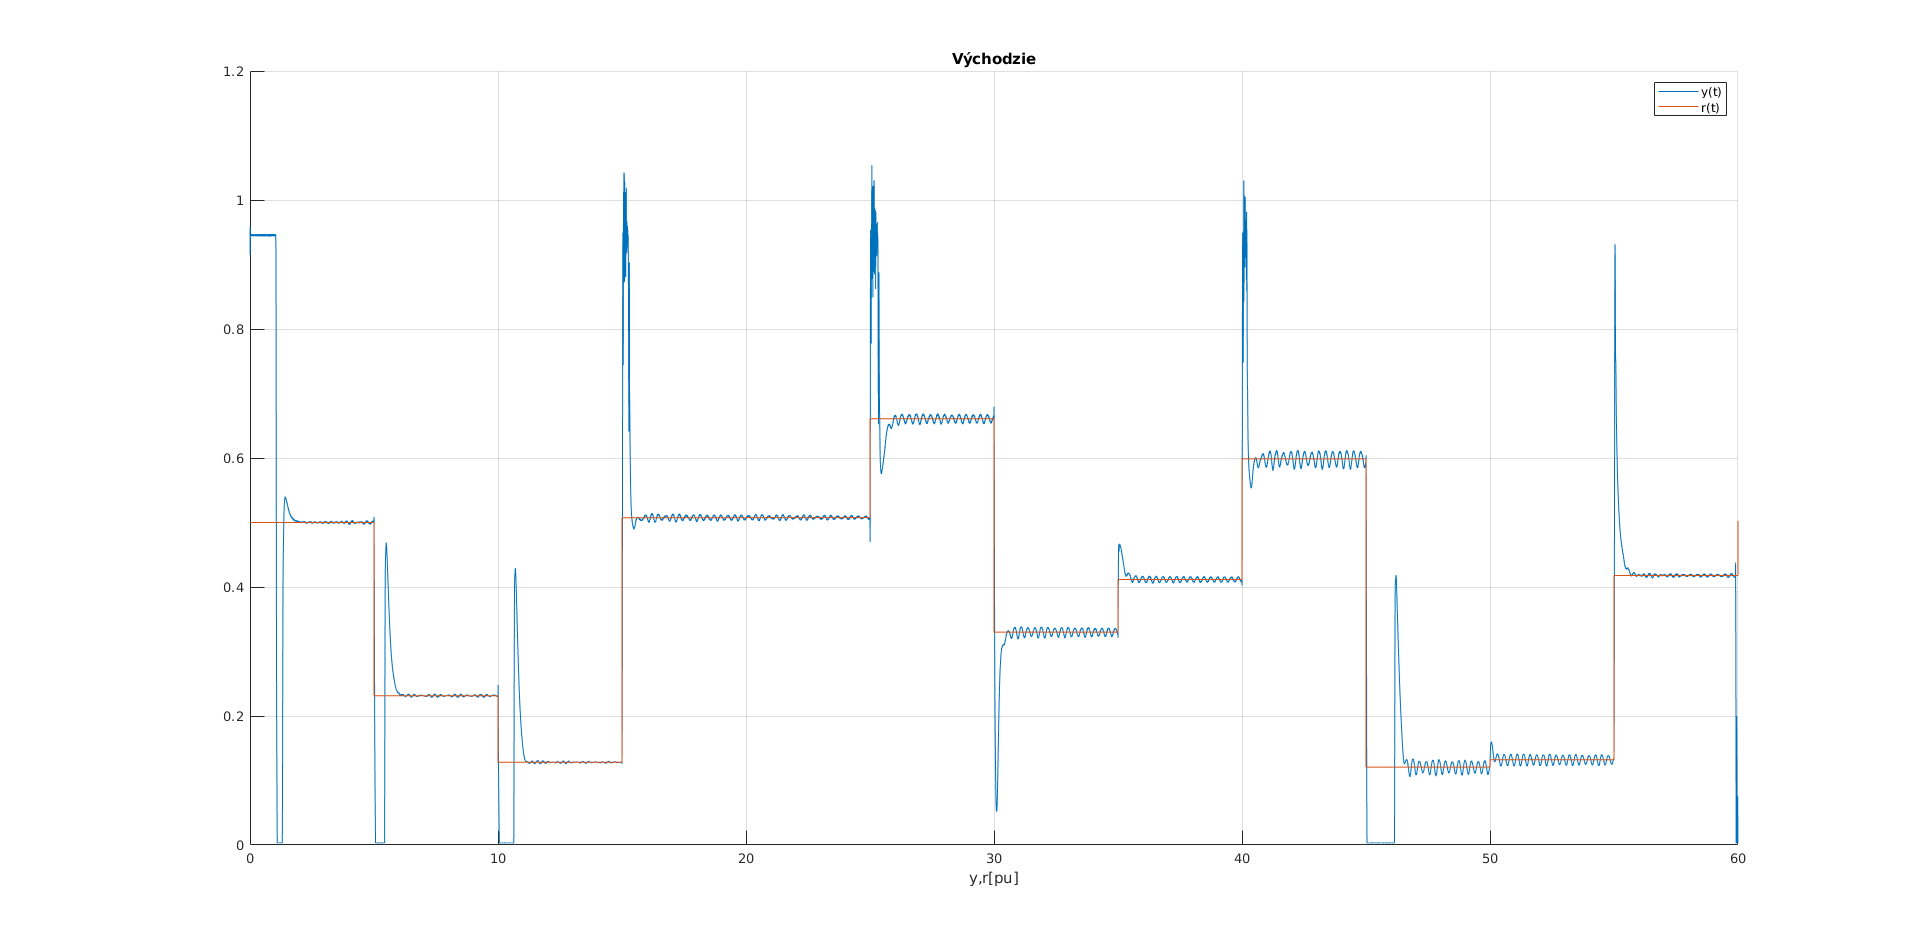
\includegraphics[width=0.8\textwidth]{./include/m6.png}
	\end{center}
	\caption{Graf štvrtého merania.}
	\label{fig:meranie4}
\end{figure}

Vo~štvrtom meraní sme zmenšili \textbf{integračnú} zložku regulátora o~20\%. Výsledok je viditeľný
na~obrázku Obr.~\ref{fig:meranie4}. Zmenšenie integračnej zložky malo za~dôsledok pomalšiu, ale~zato
presnejšiu stabilizáciu systému.

\clearpage

\subsection{Meranie 5}
\label{sec:meranie5}

\begin{table}[!htbp]
	\caption{Koeficienty PID regulátora}
	\label{tab:t5}
	\begin{center}
		\begin{tabular}[c]{|l|l|}
			\hline
			P & 1 \\
			I & 4 \\
			D & 0.0128 \\
			\hline
		\end{tabular}
	\end{center}
\end{table}

\begin{figure}[!htbp]
	\begin{center}
		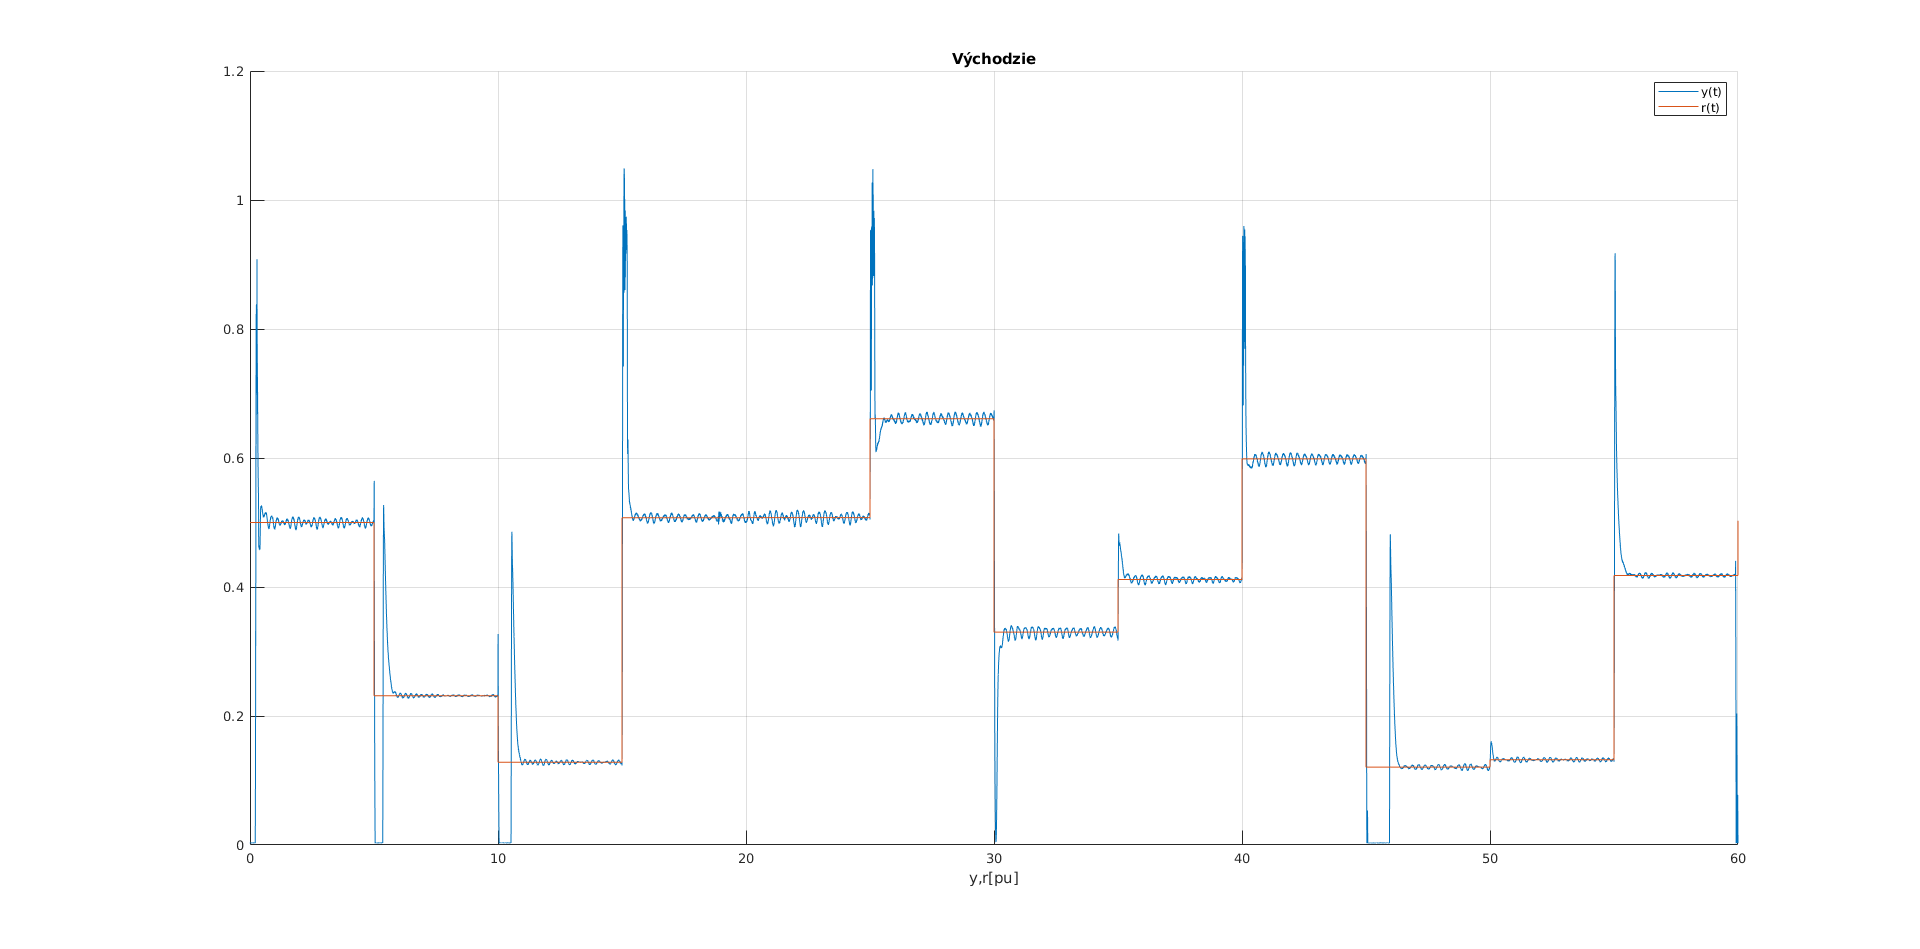
\includegraphics[width=0.8\textwidth]{./include/m5.png}
	\end{center}
	\caption{Graf piateho merania.}
	\label{fig:meranie5}
\end{figure}

V~piatom meraní sme zmenšili \textbf{derivačnú} zložku regulátora o~20\%. Výsledok je viditeľný
na~obrázku Obr.~\ref{fig:meranie5}. Zmenšenie derivačnej zložky malo za~dôsledok zmenšenie odozvy
regulátora na~zmenu výstupu. To~spôsobilo menšie prekmity v~ustálených stavoch.

\clearpage

\subsection{Meranie 6}
\label{sec:meranie6}

\begin{table}[!htbp]
	\caption{Koeficienty PID regulátora}
	\label{tab:t6}
	\begin{center}
		\begin{tabular}[c]{|l|l|}
			\hline
			P & 1 \\
			I & 4 \\
			D & 0.0192 \\
			\hline
		\end{tabular}
	\end{center}
\end{table}

\begin{figure}[!htbp]
	\begin{center}
		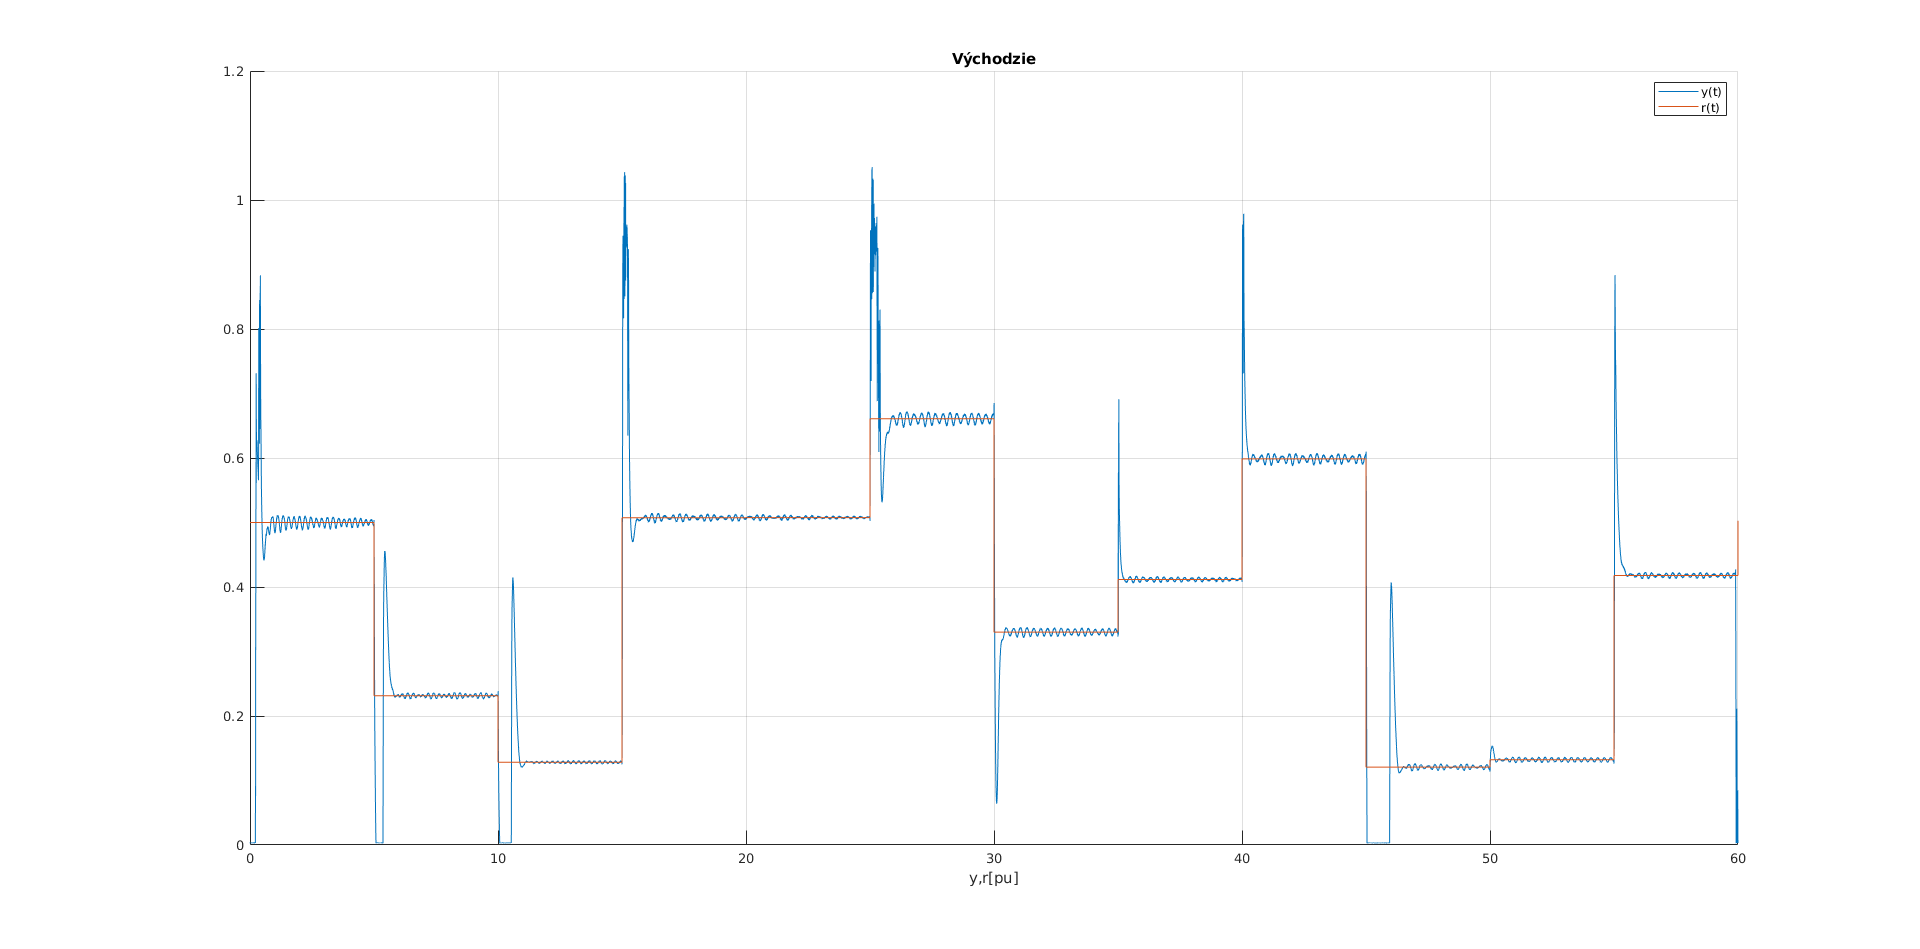
\includegraphics[width=0.8\textwidth]{./include/m7.png}
	\end{center}
	\caption{Graf šiesteho merania.}
	\label{fig:meranie6}
\end{figure}

V~šiestom meraní sme zväčšili \textbf{derivačnú} zložku regulátora o~20\%. Výsledok je viditeľný
na~obrázku Obr.~\ref{fig:meranie6}. Zväčšenie derivačnej zložky malo za~dôsledok neskoršie
ustálenie systému po~jednotkovom skoku žiadanej hodnoty. Toto je viditeľne v~45 sekunde posledného
spomínaného grafu.

\clearpage

\section{Záver}
\label{sec:zaver}

Tabuľka Tab.~\ref{tab:zaver} zobrazuje zoradenie od~najlepšieho po~najhorší skúšaný PID regulátor.
Pri~porovnávaní regulátorov sme nebrali do~úvahy prve tri skoky respektíve prvých 15 sekúnd.
Brali sme do~úvahy rýchlosť regulácie, presnosť výsku preregulovania a~ustálenosť systému
na~žiadanej hodnote.

\begin{table}[!htbp]
	\begin{center}
		\begin{tabular}[c]{|l|l|l|l|l|}
			\hline
			Meranie & P & I & D \\
			\hline
			\ref{fig:meranie1} & 1,2 & 4 & 0.016 \\
			\ref{fig:meranie5} & 1 & 4 & 0.0128  \\
			\ref{fig:meranie6} & 1 & 4 & 0.0192 \\
			\ref{fig:meranie4} & 1 & 3.2 & 0.016 \\
			\ref{fig:m1} & 1 & 4 & 0.016 \\
			\ref{fig:meranie3} & 1 & 4.8 & 0.016 \\
			\ref{fig:meranie2} & 0.8 & 4 & 0.016 \\
			\hline
		\end{tabular}
	\end{center}
	\caption{Zoradenie najlepšej funkcionality skúšaných PID regulátorov.}
	\label{tab:zaver}
\end{table}

\end{document}

